
%(BEGIN_QUESTION)
% Copyright 2006, Tony R. Kuphaldt, released under the Creative Commons Attribution License (v 1.0)
% This means you may do almost anything with this work of mine, so long as you give me proper credit

An essential component of any digital control system is an {\it analog-to-digital converter}, or {\it ADC}.  This is necessary to convert the analog process variable measurement into a digital number for the control algorithm to process.  Another essential component is a {\it digital-to-analog converter}, or {\it DAC}, which does the exact opposite.

In a system using 4-20 mA analog currents to relay instrument signals, there is an ADC located at the process variable input of the controller, and a DAC located at the output of the controller:

$$\includegraphics[width=15.5cm]{i01498x01.eps}$$

In digital ``Fieldbus'' systems, the communication is all digital, which places the ADC at the transmitter and the DAC at the transducer:

$$\includegraphics[width=15.5cm]{i01498x02.eps}$$

\filbreak

In either case, we need to ``scale'' the binary count of the ADC and DAC to their respective analog variable values.  Consider a flow control system, with a flow transmitter ranged from 0 to 200 GPM and a pneumatic control valve operating on a pressure range of 3 to 15 PSI (instrument air).  Assuming the ADC has a resolution of 16 bits (a digital conversion range of \$0000 to \$FFFF) and the DAC has a resolution of 14 bits (a digital conversion range of \$0000 to \$3FFF), determine the digital values corresponding to a 50\% PV signal (100 GPM flow rate) and a 50\% valve position (9 PSI pneumatic signal).  Write these hexadecimal number values in the following tables:

\vskip 10pt

\noindent
{\bf Calibration table for process variable signal (ADC)}

% No blank lines allowed between lines of an \halign structure!
% I use comments (%) instead, so that TeX doesn't choke.

$$\vbox{\offinterlineskip
\halign{\strut
\vrule \quad\hfil # \ \hfil & 
\vrule \quad\hfil # \ \hfil \vrule \cr
\noalign{\hrule}
%
% First row
Measurement & Digital output \cr
%
\noalign{\hrule}
%
% Another row
0 GPM & \$0000 \cr
%
\noalign{\hrule}
%
% Another row
100 GPM &  \cr
%
\noalign{\hrule}
%
% Another row
200 GPM & \$FFFF \cr
%
\noalign{\hrule}
} % End of \halign 
}$$ % End of \vbox

\vskip 10pt

\noindent
{\bf Calibration table for output signal (DAC)}

% No blank lines allowed between lines of an \halign structure!
% I use comments (%) instead, so that TeX doesn't choke.

$$\vbox{\offinterlineskip
\halign{\strut
\vrule \quad\hfil # \ \hfil & 
\vrule \quad\hfil # \ \hfil \vrule \cr
\noalign{\hrule}
%
% First row
Measurement & Digital output \cr
%
\noalign{\hrule}
%
% Another row
\$0000 & 0 PSI\cr
%
\noalign{\hrule}
%
% Another row
 & 9 PSI \cr
%
\noalign{\hrule}
%
% Another row
\$3FFF & 15 PSI\cr
%
\noalign{\hrule}
} % End of \halign 
}$$ % End of \vbox

\vskip 10pt

Note that the DAC output does {\it not} correspond to a live zero scale.  In other words, a digital input value of \$0000 will output no pressure to the valve (0 PSI), rather than a standard pneumatic ``zero'' signal of 3 PSI.

\underbar{file i01498}
%(END_QUESTION)





%(BEGIN_ANSWER)

\noindent
{\bf Calibration table for process variable signal (ADC)}

% No blank lines allowed between lines of an \halign structure!
% I use comments (%) instead, so that TeX doesn't choke.

$$\vbox{\offinterlineskip
\halign{\strut
\vrule \quad\hfil # \ \hfil & 
\vrule \quad\hfil # \ \hfil \vrule \cr
\noalign{\hrule}
%
% First row
Measurement & Digital output \cr
%
\noalign{\hrule}
%
% Another row
0 GPM & \$0000 \cr
%
\noalign{\hrule}
%
% Another row
100 GPM & {\bf \$8000} \cr
%
\noalign{\hrule}
%
% Another row
200 GPM & \$FFFF \cr
%
\noalign{\hrule}
} % End of \halign 
}$$ % End of \vbox

\vskip 10pt

\noindent
{\bf Calibration table for output signal (DAC)}

% No blank lines allowed between lines of an \halign structure!
% I use comments (%) instead, so that TeX doesn't choke.

$$\vbox{\offinterlineskip
\halign{\strut
\vrule \quad\hfil # \ \hfil & 
\vrule \quad\hfil # \ \hfil \vrule \cr
\noalign{\hrule}
%
% First row
Measurement & Digital output \cr
%
\noalign{\hrule}
%
% Another row
\$0000 & 0 PSI\cr
%
\noalign{\hrule}
%
% Another row
{\bf \$2666} & 9 PSI \cr
%
\noalign{\hrule}
%
% Another row
\$3FFF & 15 PSI\cr
%
\noalign{\hrule}
} % End of \halign 
}$$ % End of \vbox


%(END_ANSWER)





%(BEGIN_NOTES)

100 GPM = 50\% of a 0-200 GPM range.  Since the input has a 16-bit resolution (0 to 65535 counts), one-half of that is ${65535 \over 2} = 32767.5$.  Rounding down (32767) we get \$7FFF.  Rounding up (32768) we get \$8000.

\vskip 10pt

9 PSI = 60\% of a 0-15 PSI range.  Since the output has a 14-bit resolution (0 to 16383 counts), 60\% of that is $16383 \times 0.6 = 9829.8$,  Rounding down (9829) we get \$2665.  Rounding up (9830) we get \$2666.

%INDEX% Electronics review: ADC resolution
%INDEX% Electronics review: DAC resolution

%(END_NOTES)


